\chapter{Methodology}
Our method can be seen as an approach built upon the idea of leaf-root path or sub-path (section~\ref{leafrootmethod}), in an operation tree~\cite{goodsurvey}. 
But we have developed this idea further in many ways. 
Our index is composed from leaf-root paths from mathematical formulae operation tree. 
The search method is traversing a ``reversed" sub-path tree, coming along with a pruning method and a proposed sub-structure test algorithm, which are utilizing some observed properties from our indexed tree. 
Apart from these, we also offer several rules of constrains to measure symbolic similarity.
This chapter gives a summary on the method intuition and the core ideas behind these.

The methods in a nutshell is, for a document expression, construct operation tree and break it down into sub-paths, index those paths by inserting them into a tree-structured index by their reversed order. For a search query, traversal index tree as the same way of going through the reversed sub-paths of that query (search path), get the search results along the merged ways from different search paths. Finally apply symbol similarity measurement algorithm or the sub-structure test algorithm to rank results.

\section{Intuitions}
First it is beneficial to document our intuitions on using operation tree as our intermediate representation and our idea to index it in a way of “reversed” sub-path tree, and also explain in abstract why this way helps reduce index space and boost search speed.
We will give an illustrative example to describe these processes further in section~\ref{secIllu}.

\subsection{Commutative immunity}
Operators with semantic implication of commutative property (e.g. addition and multiplication) are exhaustively used in mathematical language. The ability to identify the identical equations for any permutation is very essential for a mathematical similarity search engine. 
Given this as a start point, the leaf-root paths have the advantage to cope this so that we do not need to generate different order of patterns to match formulae with commutative operator. 
To illustrate this, we know that a leaf-root path from an operation tree (see figure~\ref{oprtreeExample}) is generated through traversing in a bottom-up (or top-down) fashion from a tree, thus path string is independent with the relative position of operands from same father node.
In another word, an operation tree uniquely determines the leaf-node paths decomposed from the tree, no matter how operands are ordered. 

\subsection{Sub-structure query ability}
On the other hand, the structure of operation tree also makes it easy to represent sub-expression relation with a formula, because a sub-expression in a formula is usually (depending on the way we construct an operation tree) also a subtree in an operation tree. 
And by going up from leaves of operation tree, we are essentially traversing to an expression from its subexpression for every level. 
By making all the leaf-root paths as an index, we can search an expression by going through and beyond the leaf-root paths from its subexpression. 
This makes operation tree better in terms of searching an expression given a sub-expression in query. 
And it avoids information augmentation on index as some other structure-based methods need to do (e.g. index all sub-terms of an expression in MWS~\cite{Kohlhase06}). Therefore it helps save storage space. 

\subsection{Index and search properties}
Additionally, some properties from the ``inverted" of sub-paths (we will illustrate this in section~\ref{secIllu}) from an operation tree suggest some reduce of space and pruning possibilities in search process. 
First the sub-paths themselves can be indexed into a tree so that we can search a sub-path by traversing a sub-path tree, instead of hashing it to find a corresponding value as the symbol-pair search engine (i.e. \textit{Tangent}~\cite{symbolpairs15}) does. 
This allows us to save a lot space as the reverted sub-paths of a large collection will have a great percentage of level sharing a common string with each other. 
Also the way to search in a tree structure with a limited branch factor does not lose much efficiency compared to the HASH methods used in \textit{Tangent}, while also offer great storage efficiency.
Second, by searching from all the ``reverted" sub-paths of a query expression in our proposed index, and apply an intersection on the results from different sub-paths, we will find all the expressions have that query as subexpression (number four observed property from section~\ref{observationlabel}). And during this search process, upon going further from the query expression root in the ``reverted" sub-path, we can merge the next search directories by pruning all the entries that are not shared in common among all the ``reverted" search path directories. 
Further more, multiple index search in different path level are independent with each other, put in another way, if a given indexed formula has been found in one search path level, then its other relevant sub-paths (in terms of the current query) will most likely be found at the same search level too, thus some implementation strategies can be applied to speed search further (i.e. distributed search to quick search massive), which we would address in the next chapter.

\begin{figure}
\begin{minipage}[b]{2.65in}
\begin{center}
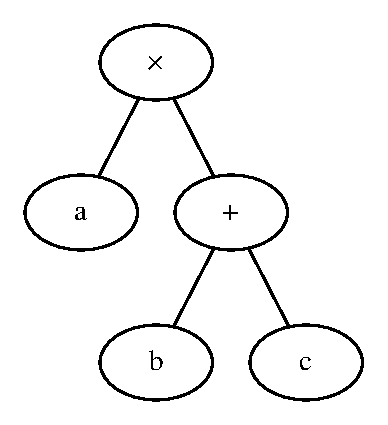
\includegraphics[height=1.8in]{leafroottree}
\\$a(b+c)$ in operation tree
\end{center}
\end{minipage}
\hspace*{.38in}
\begin{minipage}[b]{2.65in}
\begin{center}
\raisebox{.0in}{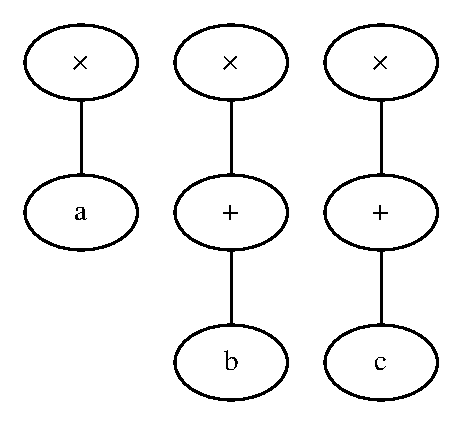
\includegraphics[height=1.8in]{leafrootpath}}
Generated leaf-root paths
\end{center}
\end{minipage}
\caption{Leaf-root path example}\label{oprtreeExample}
\end{figure}

\section{Structure Similarity}
The basic ideas used in our approach, to test whether a mathematical expression is an sub-structure of another, to prune and to constrain search process are the foundation work in our research. It is desired to give a description in a formal language so that we can deliver these ideas in the most precise way. Some important observations as well as brief justifications are provided after definitions.

\subsection{Definitions}
For the second issue addressed in section~\ref{measure_sim}, specifically, to assess the structural similarity. 
Previous formal definitions~\cite{improving09} have been given on this, providing a quantified \mbox{$n$-similarity} relation to address the similarity degree, which is determined by the max-weight common subtree between two formulae. 
The subtree, by their definition, includes all descendants from a node. 
Nevertheless, we are going to use the subtree definition in graph theory here to describe the sub-structure relation. 
To be explicit, given a rooted tree $T$, the connected graph whose edges are also in $T$ is defined as the subtree of $T$.  

Also we need clarify some conventional notations here. 
Through this paper, a path $p \in \mathbf{P}$ is a sequence of numbers given by $p = p_0 p_1 \ldots p_n$ where $n\ge0$, $p_i \in \mathbf{R},\; 0 \le i \le n$ and $\mathbf{P}$ is the set of all paths, including empty path. 
Any function $f(\cdot) = y \in \mathbf{R}$ applied on $p$ is mapped to a path too: $f(p)=f(p_0)f(p_1) \ldots f(p_n)$. 
Furthermore, for two paths $\,^1p = p_0p_1 \ldots p_n$ and $\,^2p = p_np_{n+1} \ldots p_m$ where $m \ge n$, a concatenation $\,^1p \cdot \,^2p$ is defined as $p_0p_1 \ldots p_n p_{n+1} \ldots p_m$ (said as concatenation of $\,^2p$ on $\,^1p$), 
and the concatenation of a path $p$ on a set $S = \{ s_1, s_2 \ldots s_n \}$ is defined as $S \cdot p = \{ s_1\cdot p,\  s_2\cdot p \ \ldots \ s_n\cdot p \}$. 
Usually a path with only one element is explicitly stated and wrapped by a bracket, e.g. $p=(p_0)$. 
Lastly, \textit{the longest common postfix} path $p^*$ between two path $p_1$ and $p_2$ is mapped by the function $\mathrm{lcp}$: $p^* = \mathrm{lcp}(p_1, p_2) = \mathrm{lcp}(p_2, p_1)$.

Based upon this,  we introduce a \textit{formula subtree} relation to address the sub-structure relation between two mathematical expressions. 
The formula tree is associated with a label (labels are not required to be distinct here) in each node to represent a mathematical operator, variable, constance etc., also a symbol value in each leaf node to represent a symbolic instance of that constance or variable (e.g. ``123", $\beta$, \textit{x, y} etc.). 
Below are our formal definitions.

\subsubsection{Formula tree}
A \textit{formula tree} is a labeled rooted non-empty tree $T = T(V,E,r)$ with root $r$, where each vertices $v \in V(T)$ is associated with a label $\ell_T(v) \in \mathbf{R}$ mapped by label function $\ell_T$, 
and each leaf $l \in V(T)$ is also associated with a symbol $\mathcal{S}_T(v) \in \mathbf{R}$ mapped by symbol function $\mathcal{S}_T$. For convenience, we will write $\ell$ and $\mathcal{S}$ as function names which refer to the tree implied by the context, also use function $\mathcal{S}(p)$ to indicate the symbol of the leaf in a leaf-root path $p$.

\subsubsection{Formula subtree}
\label{frmlsubtreeDef}
Given formula tree $S$ and $T$, we say $S$ is a \textit{formula subtree} of $T$ if there exists an injective mapping $\phi: V(S) \rightarrow V(T)$ satisfying:

\begin{enumerate}
\item 
$\forall\; (v_1,v_2) \in E(S)$, we have $(\phi(v_1),\phi(v_2)) \in E(T)$;
\item
$\forall\; v \in V(S)$, we have $\ell(v) = \ell(\phi(v))$;
\item
If $v \in V(S)$ is a leaf vertices in $S$, then $\phi(v)$ is also a leaf in $T$.
\end{enumerate}
Such a mapping $\phi$ is called a formula subtree isomorphic embedding (or formula embedding) for $S \rightarrow T$. 
If satisfied, we denote $S \preceq_l T$ on $\Phi$, where $\Phi$ ($\Phi \neq \emptyset$) is the set of all the possible formula embeddings for $S \rightarrow T$.

\subsubsection{Index}
An \textit{index} $\Pi$ is a set of trees such that $\forall\; T \in \Pi$, we have $T \in \mathcal{I}_{\Pi}(a)$ for any $a = \ell(p), \; p \in g(T)$, we say $T$ is indexed in $\Pi$ with respect to $a$.
Where $\mathcal{I}_{\Pi}$ is called an index look-up function. 

\subsubsection{Leaf-root path set}
Lastly, a \textit{leaf-root path set} generated by tree $T$ is a set of all the leaf-root paths from tree $T$, mapped by a function $g(T)$. Therefore we have $p \in g(T)$ for any leaf-root path $p$ of tree $T$.


\subsection{Observations}
\label{observationlabel}
We have concluded the following observations from which the interpretation can be implied that gives us some insights into the structural properties of formula tree. Our structural isomorphism test algorithm and search method are based upon these. 

\subsubsection*{Observation \#1} 
For two formula trees which satisfy $T_q \preceq_l T_d$ on $\Phi$, then $\forall\; \phi \in \Phi,\, p \in g(T_q)$, also any vertices $v$ along path $p$, the following properties are obtained:
\begin{eqnarray}
\deg(v) \le \deg(\phi(v)) \label{prop1} \\
\ell(p) = \ell(\phi(p)) \label{prop3} \\
\left| g(T_q) \right| \le \left| g(T_d) \right| \label{prop4}
\end{eqnarray}
\textit{Justification.} 
Because $\forall\; w \in V(T_q) \  s.t. \  (v, w) \in E(T_q)$, there exists $(\phi(v), \phi(w)) \in E(T_d)$. 
And for any (if exists) two different edges $(v, w_1), (v, w_2) \in E(T_q),\, w_1 \not= w_2 \in V(T_q) $, we know $(\phi(v), \phi(w_1)) \not= (\phi(v), \phi(w_2))$ by definition~\ref{frmlsubtreeDef}. 
Therefore any different edge from $v$ is associated with a distinct edge from $\phi(v)$, thus we can get (\ref{prop1}). 
Given the fact that every non-empty path $p$ can be decomposed into a series of edges $(p_0, p_1), (p_1, p_2) \ldots (p_{n-1}, p_n), \; n > 0$,
property (\ref{prop3}) is trivial.
Because there is exact one path between every two nodes in a tree, the leaf-root path is uniquely determined by a leaf node in a tree. Hence the rationale of (\ref{prop4}) can be obtained in a similar manner with that of (\ref{prop1}), expect neighbor edges are replaced by leaf-node paths.


\subsubsection*{Observation \#2} 
Given two formula trees $T_q$ and $T_d$, if $\left| g(T_q) \right| = 1$ and $\ell(g(T_{q})) \subseteq \ell(g(T_d))$, then $T_q \preceq_l T_d$.

\noindent \textit{Justification.} 
Obviously there is only single one leaf-root path in $T_q$ because $\left| g(T_q) \right| = 1$. 
Denote the path as $p = p_0 \ldots p_n,\; n \ge 0$ where $p_n$ is the leaf, and let $a = \ell(p)$.
Since $a \subseteq \ell(g(T_d))$, we know that there must exist a path $p'=p'_0 \ldots p'_n \in g(T_d)$ such that $a = \ell(p')$.
Without loss of generality, suppose $p'_n$ is the leaf of $T_d$. 
Now the injective function $\phi: p_i \rightarrow p'_i,\  0 \le i \le n$ satisfies all the requirements for $T_q$ as a formula subtree of $T_d$.

\subsubsection*{Observation \#3} 
For two formula trees $T_q$ and $T_d$, if $T_q = T(V,E,r) \preceq_l T_d$ on $\Phi$,  
$\forall a,b \in g(T_q)$ and a mapping $\phi \in \Phi$. 
Let $T_d' = \, ^{t}T_d$ where $t = \phi(r)$ and $a' = \phi(a)$, $\forall\; b' \in g(T_d')$, it follows that:
$$
\begin{array}{lcr}
b' = \phi(b)  & \Rightarrow & 
\left| \mathrm{lcp}(a,b) \right| = \left| \mathrm{lcp}(a',b') \right|
\end{array}
$$
Furthermore, $\forall\; c \in g(T_q)\; s.t.\; \left| \mathrm{lcp}(a,b) \right| \neq \left| \mathrm{lcp}(a,c) \right| $, we have
$$
\begin{array}{lcr}
\left| \mathrm{lcp}(a,b) \right| = \left| \mathrm{lcp}(a',b') \right|
& \Rightarrow &
b' \neq \phi(c)
\end{array} 
$$
\textit{Justification.} 
Because $a,b \in g(T_q)$, thus $a_0 = b_0 = r$, we make sure $\mathrm{lcp}(a,b) \ge 1$. 
Denote the path of $a = a_0 \ldots a_n a_{n+1} \ldots a_{l-1}$, similarly the path of $b=b_0 \ldots b_n b_{n+1} \ldots b_{m-1}$,
where the length of each $l,m \ge 1$ and $a_i = b_i,\, 0 \le i \le n \le \min(l-1, m-1)$ while $a_{n+1} \neq b_{n+1}$ if $l,m > 1$.
On the other hand $a' = \phi(a)$ and $b' \in g(\,^{t}T_d)$, therefore $a'_0 = \phi(a_0) = \phi(r) = t = b'_0$.
For the first conclusion, if $b' = \phi(b)$, there are two cases. If any of $|a|$ or $|b|$ is equal to one then $\left| \mathrm{lcp}(a,b) \right| = |(r)| = |(t)| = \left| \mathrm{lcp}(a',b') \right| = 1$;
Otherwise if $l,m > 1$, path $a_0 \ldots a_n = b_0 \ldots b_n$ and $a_{n+1} \neq b_{n+1}$ follow that $\phi(a_0 \ldots a_n) = \phi(b_0 \ldots b_n)$ and $\phi(a_{n+1}) \neq \phi(b_{n+1})$ by definition.
Because edge $(\phi(a_n), \phi(a_{n+1}))$ and $(\phi(b_n), \phi(b_{n+1}))$ are also in $E(T'_d)$, 
we see $\left| \mathrm{lcp}(a,b) \right| = \left| \mathrm{lcp}(a',b') \right| = n$.
For the second conclusion, we prove by contradiction. 
Assume $b' = \phi(c)$, by the first conclusion we know $\left| \mathrm{lcp}(a,c) \right| = \left| \mathrm{lcp}(a',b') \right|$.
On the other hand, because $\left| \mathrm{lcp}(a,c) \right| \neq \left| \mathrm{lcp}(a,b) \right| =  \left| \mathrm{lcp}(a',b') \right|$, 
thus $\left| \mathrm{lcp}(a,c) \right| \neq \left| \mathrm{lcp}(a',b') \right|$ which is impossible. 

\subsubsection*{Observation \#4} 
Given an index $\Pi$ and a formula tree $T_q$, $\forall\; T_d \in \Pi$:
If $T_q \preceq_l T_d$ on $\Phi$, then $\exists\; \hat{a} \in \mathbf{P},\; s.t.$
$$
T_d \in \bigcap_{a \in L} \mathcal{I}_{\Pi}(a)
$$
where $L = \ell(g(T_q)) \cdot \hat{a}$. 

\noindent \textit{Justification.} 
Denote the root of $T_q$ and $T_d$ as $r$ and $s$ respectively. 
Let $\hat{p}$ be the path determined by vertices from $t=\phi(r)$ to $s$ in $T_d$,
and $\,^1p, \,^2p \ldots \,^np,\; n \ge 1$ be all the leaf-node paths in $T_q$.
Then $\hat{a} = \ell(\hat{p})$, this is because:
$L = \ell(\{ \,^1p, \,^2p \ldots \,^np \}) \cdot \hat{a} = 
\ell(\{ \phi(\,^1p), \phi(\,^2p) \ldots \phi(\,^np) \}) \cdot \ell(\hat{p}) =
\{ \ell(\phi(\,^1p) \cdot \hat{p}), \ell(\phi(\,^2p) \cdot \hat{p}) \ldots \ell(\phi(\,^np) \cdot \hat{p}) \}
$. 
According to definition~\ref{frmlsubtreeDef} and $t=\phi(r)$, we have $\phi(\,^ip) \cdot \hat{p} \in g(T_d),\; 1 \le i \le n$.
Since $ T_d \in \Pi$, $T_d$ is indexed in $\Pi$ with respect to each of the elements in $L$, that is to say $\forall\; a \in L, \; T_d \in \mathcal{I}_{\Pi}(a)$.

\subsection{Interpretation}
\label{labelinterp}
The observations above offer some insights on how to test a substructure of a mathematical expression and how to search for an indexed mathematical expression. 

First we give some explanations on the definition.
A formula subtree relation defined in \ref{frmlsubtreeDef} describes not only a sub-structure relation between two math expressions, it also requires a label similarity and leaf inclusion.
Because structure shape (subtree isomorphic) is not only one factor to determine whether a math formula is a subexpression of another. 
Given expression in figure~\ref{oprtreeExample} as an example, where $b+c$ is an subexpression of $a \times (b+c)$, and we consider ``similar" between the two.
However, if expressions with different symbols but in similar semantics are given, e.g. $b \oplus c$ or $b \pm c$, 
they should also be considered as similar to $a \times (b+c)$ because both the operations has the similar semantical meaning as ``add". 
These operations should be labeled the value of which all the similar operation tokens are the same. 
Also, operation tree representation generally puts operator in the intermediate nodes and operands in the leaves, so it is not common to address a sub-structure without leaves, like ``$a \times + $". So a structure-similarity relation of two should also contain their leaves.

Now that we have defined our structure similarity rule as whether two trees $T_q$ and $T_d$ can satisfy: $T_q \preceq_l T_d$. We break down a formula tree into leaf-root paths $p$ and index the label of each path $\ell(p)$. So if given a ``similar" path $q$, we can further find the previous trees that also have $\ell(q)$ as its labeled path.

In section~\ref{observationlabel}, the first observation gives some constrains to test if two leaf-node paths are similar without knowing the complete tree from which they are generated.
However, comparing all the paths from the index one by one would be very inefficient. Observation \#4 suggests if we search the index by all the generated leaf-node paths from a tree at the same time, then we may just need to look into an intersected region instead of the whole collection.
Because every tree indexed ($T_d \in \Pi$) and matched by the query will be found at the intersection of index with respect to paths starting from each query leaf-root, 
furthermore, the search paths from these start points (indicated by $\ell(g(T_q))$ set), is the same (indicated by $\hat{a}$). Therefore we can ``merge" the paths ahead and prune those paths not in common. Level by level, we will finally find the matched tree.

\begin{figure}
\begin{minipage}[b]{2.65in}
\begin{center}
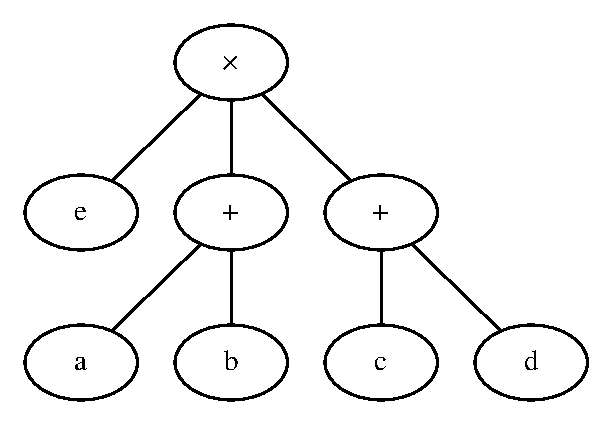
\includegraphics[height=1.8in]{not-necessary}
\\ $(a+b) \times (c+d) \times e$
\end{center}
\end{minipage}
\hspace*{.38in}
\begin{minipage}[b]{2.65in}
\begin{center}
{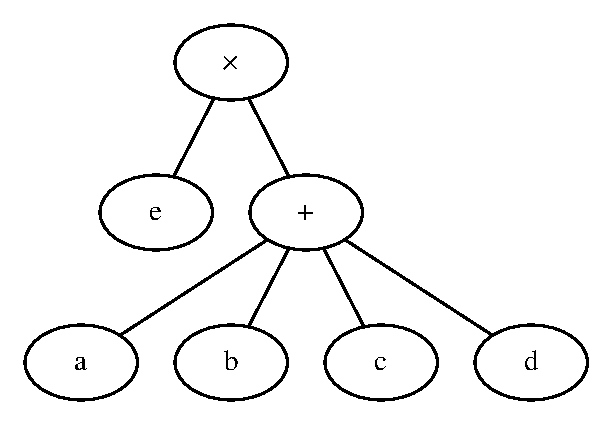
\includegraphics[height=1.8in]{not-necessary2}}
\\ $(a+b+c+d) \times e$
\end{center}
\end{minipage}
\caption{Leaf-root paths with different structure}\label{notnecessary}
\end{figure}

However, knowing the matched tree in in a set does not necessarily mean all the tree in the set match with query. 
Figure~\ref{notnecessary} gives one case where two set of leaf-root paths are identical while the structures from which they are generated are different, and not in any sub-tree relation. If left figure is the query, then we can certainly find the tree in right figure as long as it is indexed, indicated by observation \#4 in section~\ref{observationlabel}.
Although leaf-root paths offer some desired properties, whether the trees found through searching sub-paths of a query are also structure isomorphic with the query tree is still unknown. 

Observations \#2 and \#3 in section~\ref{observationlabel} offer the way to test structure isomorphic.
The former is a sufficient condition to test structure isomorphic, but the tree must first have only one leaf-root path. The latter states two necessary conditions to be a formula subtree of another.
This leads to an idea to decompose the tree and divide the problem into subtree matching problems by ruling out impossible matches between leaf-root paths using observation \#3, until it is obvious to conclude the structure isomorphic in a sub-problem by using observation \#2.

\begin{figure}
\begin{minipage}[b]{2.65in}
\begin{center}
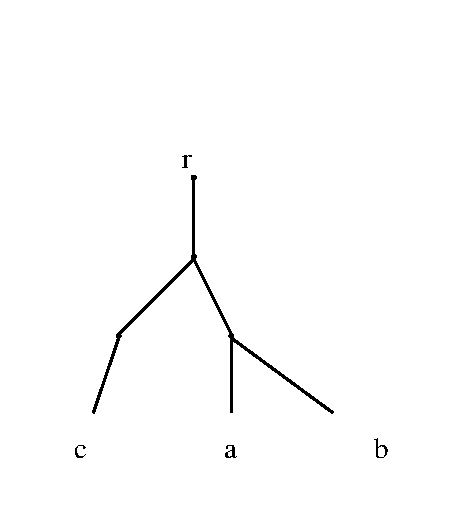
\includegraphics[height=2.8in,width=2.7in]{lpd}
\\ (a)
\end{center}
\end{minipage}
\hspace*{.38in}
\begin{minipage}[b]{2.65in}
\begin{center}
{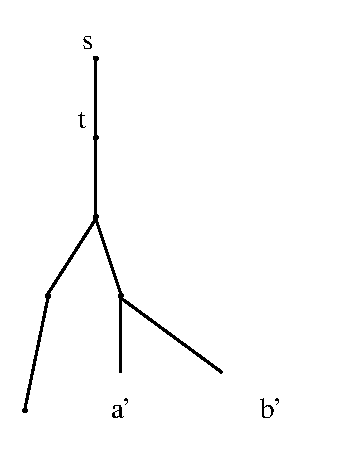
\includegraphics[height=2.8in,width=2.5in]{lpd2}}
\\ (b) 
\end{center}
\end{minipage}
\caption{Formula subtree matching}\label{submatch}
\end{figure}

\subsection{Structure match}
Here we propose and describe an algorithm for formula subtree matching based on the interpretation in section~\ref{labelinterp}.
Figure~\ref{submatch} illustrates a general case in which query tree (a) is trying to match a document tree (b).

Initially every leaf-root path in (a) should be associated with a set of leaf-root paths in (b) that are possible (by the constrains of observation~\#1 in \ref{observationlabel}) to be isomorphic, we call this set candidate set. For example the candidate set of path $a$ in (a) probably is $\{a',\ b'\}$ in (b) if the nodes are assigned universally the same label. 
Then we arbitrarily choose a path in (a) as a reference path (heuristically a \textit{heavy path}~\cite{heavypathde}), for each of the paths in its candidate set, we choose it as reference path in (b), and suppose we choose $a'$ here. At this time we can apply the two constrains from observation~\#3 and ruling out some impossible isomorphic paths in candidate set of each path in (a) and divide the problems further. 
For example, because $\left| \mathrm{lcp}(a,b) \right| = \left| \mathrm{lcp}(a',b') \right|$, we know $b'$ is still in candidate set of $b\,$; while $b'$ is not in candidate of $c$ anymore because $\left| \mathrm{lcp}(a,b) \right| \neq \left| \mathrm{lcp}(a,c) \right|$. 
After going through these eliminations for each leaf-node path (except the reference path $a$) in (a), we now have two similar subproblems: $c$ as a subtree along with its candidate set, and $b$ as a subtree along with its candidate set. 
We can apply this algorithm recursively until a very simple subproblem is encountered, that can be solved by observation~\#2. During this process, if we find any candidate set to be empty, we stop the subproblem process and change to another reference path or stop the algorithm completely if every possible reference path is evaluated.

The detailed algorithm is described in figure~\ref{submatchalgo}. 
The main procedure is \textit{decomposeAndMatch} where the argument $Q$ and $C$ is the set of leaf-root paths in query tree and the candidate sets associated with all leaf-root paths respectively.
The procedure returns SUCC if a match is found, otherwise FAIL is returned indicating no possible match.

\begin{figure}
\begin{algorithmic}[1]

\Procedure{removeCandidate}{$d,Q,C$} 
\For {$a \in Q$}
\If{$C_a = \emptyset$}
\State \textbf{return} $\emptyset$ 
\Else
\State {$C_a := C_a - \{d\}$} 
\EndIf
\EndFor
\State \textbf{return} $C$
\EndProcedure

\State {}

\Procedure{match}{$a, a', Q, C$}
\For {$b \in Q$}
\State $t := \mathrm{lcp}(a,b)$
\State $Q_t := Q_t \cup \{b\}$
\State $P := P \cup \{t\}$
\EndFor
\For {$t \in P$}
\For {$b \in Q_t$}
\For {$b' \in C_b$}
\If {$t \not= \mathrm{lcp}(a',b')$} 
\State $C := $ \Call{removeCandidate}{$b', Q_t, C$}
\If {$|C| = 0$} 
\State \textbf{return} FAIL
\EndIf
\EndIf
\EndFor
\EndFor
\If {\Call{decomposeAndMatch}{$Q_t, C$} = FAIL} 
\State \textbf{return} FAIL
\EndIf
\EndFor
\State \textbf{return} SUCC 
\EndProcedure

\State {}

\Procedure{decomposeAndMatch}{$Q, C$}
\If {$Q = \emptyset$} \textbf{return} SUCC 
\EndIf
\State $a$ := OnePathIn(Q)
\Comment{Choose a reference path in Q}
\State $Q_{\mathrm{new}} := Q - \{a\}$
\For {$a' \in C_a$}
\State $C_{\mathrm{new}} := $ \Call{removeCandidate}{$a', Q_{\mathrm{new}}, C$}
\If {$C_{\mathrm{new}} = \emptyset$} \textbf{return} FAIL 
\EndIf
\If {\Call{match}{$a, a', Q_{\mathrm{new}}, C_{\mathrm{new}}$}}
\textbf{return} SUCC 
\EndIf
\EndFor
\State \textbf{return} FAIL
\EndProcedure

\end{algorithmic}
\caption{The decompose-and-match algorithm}\label{submatchalgo}
\end{figure}

\section{Symbolic Similarity}
Until now, we have not addressed symbolic similarity yet. 
Although mathematical expression often use symbols interchangeably, symbolic matches is a good way to differentiate similarity, and most importantly, measure some semantic similarity in mathematical language.

Firstly, structure similarity of math expression is either boolean match (subtree or not) or measured with the similarity degree only depend on the subtree depth where expressions are matched. Symbolic similarity will introduce more factors to further distinguish similarity among structural identical math expressions.
Also it is essential to give those with symbolic matches a higher rank because they may imply more semantic similarity. 
For example, $E=mc^2$ is considered more meaningful when exact symbols are used rather than just being structure identical with $y=ax^2$.

Secondly, as illustrated in section~\ref{measure_sim}, same mathematical symbols in an expression (or bound variables) usually can only maintain semantical equality if the changes are made by substitutions. (similar to the notion of $\alpha$-equality~\cite{Hindley1986}). This is an important semantic information that we need to capture and certainly it involves comparison of symbols. 

Yet there is one thing to notice here, in many mathematical search systems, a query may be specified with wildcards and thus will match any document with an expression substitution to that wildcard. 
And a query symbol not specified by wildcard is expecting an exact symbolic occurrence in document.
We are not considering wildcards here with the limitation of our substructure matching method. 
And in terms of symbolic wildcard, we also doubt the its demand in mathematical search as it is not common to expect an exact symbol occurrence when we query in mathematical language (also addressed in \cite{mias11a}).

\subsection{Ranking constrains}
As we have discussed, symbolic similarity is essential to be captured, in order to further rank document expressions. 
Here we propose two constrains to addressed all the considerations, they can be summarized as:

\begin{itemize}
\item A document expression with both structure and symbol matches (not necessarily all the symbols) is considered more relevant than that with only structure matches. 
And the more symbol matches, the more relevant it is.
\item Expressions with identical symbols at the same place (i.e. bound variable) should be considered more similar than those with different symbols at the same position. 
\end{itemize}

In this paper, we use these two constrains as the rule to rank retrieval results in terms of symbolic similarity.
And in cases where both constrains can be applied, we prioritize the second constrain. 
This is because, intuitively, as long as the semantic meaning of two expressions is the same, using different set of symbols does not make a difference. 
However, bound variable match is more important because an mathematical expression with more than one identical symbols most often imply that those symbols represents the same variable. 
Missing one or more symbols being identical will lose semantics in a certain degree.

The constrains and idea above are illustrated by the following example. 
Let the rank of a document math expression $d$ be $r(d)$, and given query $\sqrt a (a - b)$ for instance. 
It is easy to see under the first constrain: 
$$
r\big(\sqrt a (a - b)\big) > r\big(\sqrt a (a - x)\big) > r\big(\sqrt x (x - y)\big)
$$
The one with the highest rank here is an exact match, with three symbols matching in total. 
The second one has two symbols match while the third one has no symbolic match at all. 

In the same manner, by the second constrain we have:
$$
r\big(\sqrt x (x - b)\big) > r\big(\sqrt x (y - b)\big)
$$
The first one uses bound variable $x$ but it preserves the same semantics except for the symbol of bound variable is different with that of query.
The second one does not have bound variable match, in another word, it uses different symbols (i.e. ``$x,\ y$") at positions where query expression uses the same symbols (i.e. ``$a$").

One common pattern the first example follows is they all have the bound variable match. 
And for the second example, they have the same number of symbol matches (only ``$b$" is matched in a symbolic way). 
So it is easy to follow only one of the two constrain. 
However, sometimes both constrains can be applied where conflict may occur and we have to choose only one to follow. 
Given document expression $\sqrt a (x - b)$ and $\sqrt x (x - b)$ for instance, the former has two symbolic matches (i.e. ``$a,\ b$") while does not have bound variable match. The latter, on the other hand, has bound variable match while only has one symbolic match (i.e. ``$b$"). We nevertheless score the latter higher because it does not lose any semantics. 

\subsection{An algorithm}
Here we propose an algorithm to score symbolic similarity between query and document expressions.
To follow all the constrains and issues addressed, intuitively, we first take the bound variable with greatest number of occurrence, e.g. ``$a$" with three occurrences in $\left(b \cdot \dfrac{a+b}{a+c} + a\right)$, to match as many as symbols of each bound variable in a document expression in a greedy way. 
Whenever a symbol in document expression is matched, we exclude it from matching candidates in future iterations.
In the next iteration, we choose the bound variable with the second number of occurrence and repeat this process until all the query bound variable are looped.

\begin{figure}
\begin{algorithmic}[1]

\Procedure{markAndCross}{$D,Q,C$} 
\State score := 0

\If {$D = \emptyset$} 
\State \textbf{return} 0 
\EndIf
\For {$a' \in D$}
\State $T_{a'} := \mathrm{unmark}$ 
\EndFor
\For {$v \in V(D)$}
\State $B_v := 0$ 
\EndFor

\State QList := \Call{sortBySymbolAndOccur}{Q}

\For {$a$ {\bf in} QList}

\For {$v \in V(D)$}
\State $m := -\infty$
\State $m_p := \varnothing$
\For {$a' \in C_a \cap \{ y \mid y = v,\ y \in V(D)\} $}
\If {$T_{a'} = \mathrm{unmark}$ {\bf and} $\mathrm{sim}(a, a') > m$} 
\State $m := \mathrm{sim}(a, a')$ 
\State $m_p := a'$ 
\EndIf
\EndFor
\If {$m_p \not= \varnothing$}
\State $T_{m_p} := \mathrm{mark}$ 
\State $B_v := B_v + m$
\Else
\Comment{Exhausted all candidates}
\State \textbf{return} 0 
\EndIf
\EndFor

\If {$\mathcal{S}(a) \mathrm{\ has\ changed}$ {\bf or} $\mathrm{\ last\ iteration\ of\ } a$}
\label{line_bond_finish}

\State $m := -\infty$
\State $m_v := \varnothing $
\For {$v \in V(D)$}
\If {$B_v > m$} 
\State $m := B_v$ 
\State $m_v := v$ 
\EndIf
\State $B_v := 0$ 
\EndFor
\State $\mathrm{score} := \mathrm{score} + m$ 

\For {$v \in V(D)$}
\If {$v = m_v$} 
\State $\mathrm{nextState} := \mathrm{unmark}$ 
\Else
\State $\mathrm{nextState} := \mathrm{cross}$ 
\EndIf
\For {$a' \in C_a \cap \{ y \mid \{ y \mid y = v,\ y \in V(D)\} $}
\If {$T_{a'} = \mathrm{mark}$} 
\State $T_{a'} := \mathrm{nextState}$ 
\EndIf
\EndFor
\EndFor

\EndIf

\EndFor

\State \textbf{return} score
\EndProcedure

\end{algorithmic}
\caption{The mark-and-cross algorithm}\label{markcrossalgo}
\end{figure}

The algorithm is described in figure~\ref{markcrossalgo}. It takes three arguments, the set of leaf-root paths $D$ and $Q$ in document expression and query expression respectively, and the candidate sets $C$ associated with all leaf-root paths. 
The bound variables in $D$ is defined by a set $V(D) = \{x \mid \mathcal{S}(x),\ x \in D\}$, which contains all the leaf node symbols from document expression.
Function \textit{sortBySymbolAndOccur} takes the elements from a set of leaf-root paths and return a list of all the leaf-root paths, each path $p$ is ordered by the tuple $(\mathcal{S}(p), O_p)$ in the list, where $O_p$ is the number of occurrence of path $p$ in the set. 
Take the example expression $\left(b \cdot \dfrac{a+b}{a+c} + a\right)$ again, the result list returned by \textit{sortBySymbolAndOccur} is a sequence of leaf-root path of $a,a,a,b,b,c$ respectively.
Each document path $a'$ is associated with a tag $T_{a'}$ which has three possible state: marked, unmarked and crossed. And bound variable $v \in V(D)$ can be given a score $B_v$ which represents the similarity degree between two bound variables. 
The symbolic similarity function $\mathrm{sim}(a,a')$ measures the similarity degree between two leaf-root paths $a$ and $a'$. 
Intuitively, we set the similarity function:
$$
\mathrm{sim}(a,a') = 
\left\{
\begin{array}{ll}
1    &\qquad \mathrm{if}\  \mathcal{S}(a) = \mathcal{S}(a')
\\
\\
\alpha < 1  &\qquad \mathrm{otherwise}
\end{array}
\right.
$$
to give greater (double) weight to leaf-root paths with exact symbol match than those without symbol match but in a candidate set
(this function is called only when a document path is in candidate set, see figure~\ref{markcrossalgo}).
Furthermore, denote the number of variables in a bound variable $x$ in query expression that best matches the bound variable $y$ in document expression as $n_{x,y}$, 
then for the bound variable $a$ in query expression and two bound variable $a$ and $b$ in document expression, if $n_{a,b} > n_{a,a}$ then we weight the bound variable matching of $a$ in query with $b$ in document more than that of $a$ in query with $a$ in document, even if the latter has exact symbol matches.
For example, for query expression $a+\dfrac 1 a + \sqrt{a}$ and document expression $a+\dfrac 1 a + b + \dfrac 1 b + \sqrt{b}$, we have bound variable matching $\fbox{a}+\dfrac 1 {\fbox{a}} + \sqrt{\fbox{a}}$ with $a+\dfrac 1 a + \fbox{b} + \dfrac 1 {\fbox{b}} + \sqrt{\fbox{b}}$ weighted more than exact symbol matching $\fbox{a}+\dfrac 1 {\fbox{a}} + \sqrt{a}$ with $\fbox{a}+\dfrac 1 {\fbox{a}} + b + \dfrac 1 b + \sqrt{b}$
(expressions surrounded by a box indicate the matching part),
because the former matching has more variables involved even if they are not symbolic identical with its counterpart. 
That is to say, given a bound variable matching with $k$ variables of that bound variable in query, we need $\alpha$ to satisfy $ k \alpha > k-1 $
and $\alpha < 1$. In our practice, we set $\alpha$ to a value close to $1$, like $0.9$ for instance.

By sorting the query paths $Q$, the algorithm is able to take out paths from same bound variable in maximum-occurrence-first order from QList. 
Each query path $a$ tries to match a path $a'$ in each document bond variable $v$ by selecting the unmarked path $m_p$ with maximum $\mathrm{sim}(a,a')$ value, and accumulate the value on $B_v$ indicating the similarity between currently evaluating query bond variable and the bond variable $v$.
In addition, mark the tag $T_{m_p}$ associated with the document path $m_p$ which has maximum similarity value.
Once a query bond variable has been iterated (line~\ref{line_bond_finish}),
we find the document variable $m_v$ with greatest $B_v$ value $m$, and regard it as the best match bond variable in document for the bond variable just iterated, and use $m$ to contribute total score.
Before iterating a new query bond variable, we will cross all the document paths of variable $m_v$ to indicate they are confirmed been matched, 
and rollback those marked paths that are not variable $m_v$ to be unmarked.
We continue doing so until all the query path is iterated, and finally return the score indicating the symbolic similarity between query and document expression.

\section{Combine the Two}
We have already discussed and proposed the problem and algorithms to both test structure isomorphic and measure symbolic similarity between mathematical expressions. The two algorithms, however, do not cooperate in an unified way. 
To illustrate this point, assume we first use decompose-and-match algorithm and have concluded one is a formula subtree of another, but we only get one possible substructure match. 
There are very likely other possible positions where this tree can also be formula subtree of another, because the candidate sets are not unique. 
Thus we need to exhaust all possibilities and apply mark-and-cross algorithm to each of them, in order to find the maximum symbolic similarity pair. 
Analogously, assume we first want to get the symbolic similarity degree, then we are uncertain about the paths we have specified in candidate set are really isomorphic paths to the query path. 
We will not guarantee substructure relation before using decompose-and-match algorithm.

One possible way to both test strict structure isomorphism and measure symbolic similarity is to decompose the tree trying to match all the substructures but at the same time heuristically choose reference paths to achieve best symbolic similarity in a greedy way, if no possible substructure can be matched isomorphically, we have to rollback and try other candidates using backtracking.
Because the mark-and-cross algorithm has an worst case time complexity of $O\big(|Q| \times |D|\big)$,
trying to find the maximum point while introduce more parameters (we try to find the one with not only the most symbolic similarity but also who satisfies structure isomorphism) would lead to even more time complexity. 

\subsection{Relaxed structure match}
The complexity introduced to combine the two methods will make our approach infeasible to efficiently deal with large data set. 
Here we choose to relax our constrain on strict structure isomorphism. 
As figure~\ref{notnecessary} has illustrated, we know that the labels of a leaf-node path set being a subset of that of another does not necessarily mean the tree generating the former path set is a formula subtree of that generating the latter.
To further generalize it, we say for any two formula tree $T_q$ and $T_d$ and $\forall\; \hat{a} \in \mathbf{P}$, if $\ell(g(T_q)) \cdot \hat{a} \subseteq \ell(g(T_d))$, it is not sufficient to imply $T_q \preceq_l T_d$.
Nevertheless, we think the cases which makes the above statement insufficient are fairly rare in common mathematical content, and the complexity introduced from considering those cases will offset the benefit to strictly identify the structure isomorphism.
Therefore, we loose our constrain on structure similarity so that any  $T_d \in \bigcap_{a \in L} \mathcal{I}_{\Pi}(a) $ is considered structurally relevant to query formula tree $T_q$ in observation~\#4 of section~\ref{observationlabel},
and we say $T_d$ is \textit{searchable} by $T_q$ in index $\Pi$.
Optionally, we can apply constrain \ref{prop1} in observation \#1 to further eliminate cases such as the one in figure~\ref{notnecessary} thus less query/document expressions that are not in formula subtree relation would be considered relevant. We name this constrain as \textit{fan-number constrain}.

The revised method will collect all the ``structure similar" document formula trees that satisfy the fan-number constrain in the set $\bigcap_{a \in L} \mathcal{I}_{\Pi}(a)$. 
Then use mark-and-cross algorithm to finally rank the collected set by symbolic similarity.

\subsection{Matching-depth}
On the other hand, we may introduce a \textit{matching-depth factor} into symbolic similarity measurement algorithm, to make it also consider some structurally matching depth. 
As it is addressed in \cite{mias11a}, the deeper level at where two formula matches, the lower similarity weight would it be, since the deeper sub-formulae in in mathematical expression will make it less important to the overall formula.
For example, given query formula $\sqrt a$, expression $\sqrt {x}$ would score higher than $\sqrt{\sqrt{x}}$ does. 

To reflect the depth where two math expressions matches, we introduce the matching-depth factor $f(d)$ and modify the similarity function in the mark-and-cross algorithm:
$$
\mathrm{sim}(a,a') = 
\left\{
\begin{array}{ll}
f(d)   &\qquad \mathrm{if}\  \mathcal{S}(a) = \mathcal{S}(a')
\\
\\
f(d) \cdot \alpha  &\qquad \mathrm{otherwise}
\end{array}
\right.
$$
where the factor value $f(d)$ is in a negative correlation with matching depth $d = |\hat{a}|$ (See observation~\#4 of section~\ref{observationlabel}). 
Many possible functions may be adopted, we use $f(d) = \dfrac{1}{1 + d}$ in our method. 

The idea behind this is because we accumulate $\mathrm{sim}(a,a')$ value to contribute the overall symbolic similarity score returned by algorithm~\ref{markcrossalgo}. In order to incorporate mark-and-cross algorithm, by distributivity, we can distribute the factor of matching depth for two mathematical expressions, over all the path pairs generated from the two expressions. 

\subsection{Matching-ratio}
Before matching-depth is introduced, if a formula subtree relation is inferred between two formula trees, they are considered structurally matching in a boolean manner. 
There is no similarity degree between a complete match (or a sub-formula) and structurally irrelevant. 
In another word, structural differences is considered in a way to filter indexed expressions, for further symbolic similarity assessment. 
The final output ranking is determined by symbolic similarity degree, without considering structural similarity. 
Here we introduce another metres that measures the structural similarity, combined with symbolic similarity to rank final search results.

According to the property \ref{prop4} in section~\ref{observationlabel} (observation~\#1), for two expression in formula subtree relation, we have $\dfrac{|g(T_q)|}{|g(T_d)|} \le 1$, and the ratio of left-hand is named as \textit{matching-ratio}, which characterises the structural coverage for a matching query in an expression.
Consider the scenario where a query expression is structural isomorphic to two document expressions, and the symbolic similarity between them are the same. 
However, the different ratio of the document expression ``area'' to the ``area'' which the matching query covers essentially makes them scored differently.
For example, for query $ax + b$, document expression $ax + b$ should precede $x^2 + ax + b$ although the query matches both two document expressions with same symbolic score.
Therefore, in addition to the symbolic similarity degree $s$ given by mark-and-cross algorithm, we combine matching-ratio $r$ to score overall similarity and rank document expressions by the tuple $(s, r)$, that is, first compare $s$ and then compare $r$ if $s$ is equal, to rank document expressions.

\subsection{Illustrated by an example}
\label{secIllu}

We illustrate the method introduced in this chapter by a simple example here. 
Given a query expression $ax(a+b)$ and document expression $ax + (b+a)by$, here we show how we search the relevant document using this query and how the relevance score between them is calculated by mark-and-cross algorithm.

The query expression and document expression are represented by operation trees $T_q$ and $T_d$ in figure~\ref{expGraph}, 
instead of only denoting the operation symbols at the internal nodes and the variable (also can be a constant) symbols at the leaf nodes, we use the notation $^i_l S$ to denote a node with symbol $S$ labeled by $l$ (i.e. $\ell(S)=l$) with vertex number $i$. 
The three different possible labels here are $v,\ t$ and $a$, standing for unified name ``variable", ``times" and ``add" respectively.
To be concise and descriptive, we will interchangeably use either $^i_l S$ notation or $q_i$ ($p_i$) to represent the leaf-root path in a query (document) operation tree where the leaf vertex $i$ resides.

Firstly, the generated path sets for $T_q$ and $T_d$ are:
$$
\begin{aligned}
g(T_q) &= \{ 1\cdot6,\; 2\cdot6,\; 3\cdot5\cdot6,\; 4\cdot5\cdot6\} \\
g(T_d) &= \{ 5\cdot8\cdot10,\; 6\cdot8\cdot10,\; 3\cdot7\cdot8\cdot10,\; 4\cdot7\cdot8\cdot10,\; 1\cdot9\cdot10,\; 2\cdot9\cdot10\}
\end{aligned}
$$
And the labeled path sets for each of the two are:
$$
\begin{aligned}
\ell\left(g(T_q)\right) &= \{ v\cdot t,\; v\cdot a\cdot t \} \\
\ell\left(g(T_d)\right) &= \{ v\cdot t\cdot a,\; v\cdot a\cdot t \cdot a \}
\end{aligned}
$$
Because $\ell\left(g(T_q)\right) \cdot a = \ell\left(g(T_d)\right)$, or equivalently 
$$
\ell(g(T_q)) \cdot \hat{a} \subseteq \ell(g(T_d))
$$
where $\hat{a} = a$, 
we know $T_d$ is searchable by $T_q$, so we will find a path $\hat{a}$ to append after the labeled path set $\ell\left(g(T_d)\right)$ in index $\Pi$ and obtain $T_d$ to be considered as structurally relevant to $T_q$.
We can also infer the matching-depth $d$ here is $|\hat{a}| = 1$. 

\begin{figure}
\begin{minipage}[b]{2.65in}
\begin{center}
\resizebox{2.4in}{!}{
%%%%%%%%%%%%%%%%%%%%%%%%%%%%%%%%%%%%%%%%%%%%%%%%
% \begin{tikzpicture}[anchor=mid,>=latex',line join=bevel,]
\begin{tikzpicture}[>=latex',line join=bevel,]
  \pgfsetlinewidth{1bp}
\Huge%
\begin{scope}
  \pgfsetstrokecolor{black}
  \definecolor{strokecol}{rgb}{1.0,1.0,1.0};
  \pgfsetstrokecolor{strokecol}
  \definecolor{fillcol}{rgb}{1.0,1.0,1.0};
  \pgfsetfillcolor{fillcol}
  \filldraw (0bp,0bp) -- (0bp,180bp) -- (234bp,180bp) -- (234bp,0bp) -- cycle;
\end{scope}
\begin{scope}
  \pgfsetstrokecolor{black}
  \definecolor{strokecol}{rgb}{1.0,1.0,1.0};
  \pgfsetstrokecolor{strokecol}
  \definecolor{fillcol}{rgb}{1.0,1.0,1.0};
  \pgfsetfillcolor{fillcol}
  \filldraw (0bp,0bp) -- (0bp,180bp) -- (234bp,180bp) -- (234bp,0bp) -- cycle;
\end{scope}
  \pgfsetcolor{black}
  % Edge: ad5 -- b4
  \draw [] (179.35bp,72.765bp) .. controls (185.17bp,61.456bp) and (192.89bp,46.437bp)  .. (198.7bp,35.147bp);
  % Edge: ti6 -- a1
  \draw [] (84.43bp,146.83bp) .. controls (72.02bp,134.77bp) and (54.269bp,117.51bp)  .. (41.796bp,105.38bp);
  % Edge: ad5 -- a3
  \draw [] (162.65bp,72.765bp) .. controls (156.83bp,61.456bp) and (149.11bp,46.437bp)  .. (143.3bp,35.147bp);
  % Edge: ti6 -- ad5
  \draw [] (113.57bp,146.83bp) .. controls (125.98bp,134.77bp) and (143.73bp,117.51bp)  .. (156.2bp,105.38bp);
  % Edge: ti6 -- x2
  \draw [] (99bp,143.7bp) .. controls (99bp,132.85bp) and (99bp,118.92bp)  .. (99bp,108.1bp);
  % Node: b4
\begin{scope}
  \definecolor{strokecol}{rgb}{0.0,0.0,0.0};
  \pgfsetstrokecolor{strokecol}
  \draw (207bp,18bp) ellipse (27bp and 18bp);
  \draw (207bp,18bp) node {$^4_v b$};
\end{scope}
  % Node: ad5
\begin{scope}
  \definecolor{strokecol}{rgb}{0.0,0.0,0.0};
  \pgfsetstrokecolor{strokecol}
  \draw (171bp,90bp) ellipse (27bp and 18bp);
  \draw (171bp,90bp) node {$^5_a +$};
\end{scope}
  % Node: ti6
\begin{scope}
  \definecolor{strokecol}{rgb}{0.0,0.0,0.0};
  \pgfsetstrokecolor{strokecol}
  \draw (99bp,162bp) ellipse (27bp and 18bp);
  \draw (99bp,162bp) node {$^6_t \times$};
\end{scope}
  % Node: a1
\begin{scope}
  \definecolor{strokecol}{rgb}{0.0,0.0,0.0};
  \pgfsetstrokecolor{strokecol}
  \draw (27bp,90bp) ellipse (27bp and 18bp);
  \draw (27bp,90bp) node {$^1_v a$};
\end{scope}
  % Node: a3
\begin{scope}
  \definecolor{strokecol}{rgb}{0.0,0.0,0.0};
  \pgfsetstrokecolor{strokecol}
  \draw (135bp,18bp) ellipse (27bp and 18bp);
  \draw (135bp,18bp) node {$^3_v a$};
\end{scope}
  % Node: x2
\begin{scope}
  \definecolor{strokecol}{rgb}{0.0,0.0,0.0};
  \pgfsetstrokecolor{strokecol}
  \draw (99bp,90bp) ellipse (27bp and 18bp);
  \draw (99bp,90bp) node {$^2_v x$};
\end{scope}
%
\end{tikzpicture}
%%%%%%%%%%%%%%%%%%%%%%%%%%%%%%%%%%%%%%%%%%%%%%%%
} 
\\[5mm]
query expression $ax(a+b)$
\end{center}
\end{minipage}
\hspace*{.18in}
\begin{minipage}[b]{2.65in}
\begin{center}
\resizebox{3.3in}{!}{
%%%%%%%%%%%%%%%%%%%%%%%%%%%%%%%%%%%%%%%%%%%%%%%%
\begin{tikzpicture}[>=latex',line join=bevel,]
  \pgfsetlinewidth{1bp}
\Huge%
\begin{scope}
  \pgfsetstrokecolor{black}
  \definecolor{strokecol}{rgb}{1.0,1.0,1.0};
  \pgfsetstrokecolor{strokecol}
  \definecolor{fillcol}{rgb}{1.0,1.0,1.0};
  \pgfsetfillcolor{fillcol}
  \filldraw (0bp,0bp) -- (0bp,252bp) -- (342bp,252bp) -- (342bp,0bp) -- cycle;
\end{scope}
\begin{scope}
  \pgfsetstrokecolor{black}
  \definecolor{strokecol}{rgb}{1.0,1.0,1.0};
  \pgfsetstrokecolor{strokecol}
  \definecolor{fillcol}{rgb}{1.0,1.0,1.0};
  \pgfsetfillcolor{fillcol}
  \filldraw (0bp,0bp) -- (0bp,252bp) -- (342bp,252bp) -- (342bp,0bp) -- cycle;
\end{scope}
  \pgfsetcolor{black}
  % Edge: ad0 -- ti8
  \draw [] (192.43bp,218.83bp) .. controls (180.02bp,206.77bp) and (162.27bp,189.51bp)  .. (149.8bp,177.38bp);
  % Edge: ti9 -- a1
  \draw [] (243bp,143.7bp) .. controls (243bp,132.85bp) and (243bp,118.92bp)  .. (243bp,108.1bp);
  % Edge: ad7 -- b4
  \draw [] (179.35bp,72.765bp) .. controls (185.17bp,61.456bp) and (192.89bp,46.437bp)  .. (198.7bp,35.147bp);
  % Edge: ti8 -- b5
  \draw [] (116.19bp,148.81bp) .. controls (96.365bp,135.96bp) and (65.338bp,115.85bp)  .. (45.597bp,103.05bp);
  % Edge: ti9 -- x2
  \draw [] (257.57bp,146.83bp) .. controls (269.98bp,134.77bp) and (287.73bp,117.51bp)  .. (300.2bp,105.38bp);
  % Edge: ad7 -- a3
  \draw [] (162.65bp,72.765bp) .. controls (156.83bp,61.456bp) and (149.11bp,46.437bp)  .. (143.3bp,35.147bp);
  % Edge: ti8 -- y6
  \draw [] (126.65bp,144.76bp) .. controls (120.83bp,133.46bp) and (113.11bp,118.44bp)  .. (107.3bp,107.15bp);
  % Edge: ti8 -- ad7
  \draw [] (143.35bp,144.76bp) .. controls (149.17bp,133.46bp) and (156.89bp,118.44bp)  .. (162.7bp,107.15bp);
  % Edge: ad0 -- ti9
  \draw [] (215.35bp,216.76bp) .. controls (221.17bp,205.46bp) and (228.89bp,190.44bp)  .. (234.7bp,179.15bp);
  % Node: b4
\begin{scope}
  \definecolor{strokecol}{rgb}{0.0,0.0,0.0};
  \pgfsetstrokecolor{strokecol}
  \draw (207bp,18bp) ellipse (27bp and 18bp);
  \draw (207bp,18bp) node {$^4_v b$};
\end{scope}
  % Node: ti8
\begin{scope}
  \definecolor{strokecol}{rgb}{0.0,0.0,0.0};
  \pgfsetstrokecolor{strokecol}
  \draw (135bp,162bp) ellipse (27bp and 18bp);
  \draw (135bp,162bp) node {$^8_t \times$};
\end{scope}
  % Node: ti9
\begin{scope}
  \definecolor{strokecol}{rgb}{0.0,0.0,0.0};
  \pgfsetstrokecolor{strokecol}
  \draw (243bp,162bp) ellipse (27bp and 18bp);
  \draw (243bp,162bp) node {$^9_t \times$};
\end{scope}
  % Node: ad0
\begin{scope}
  \definecolor{strokecol}{rgb}{0.0,0.0,0.0};
  \pgfsetstrokecolor{strokecol}
  \draw (207bp,234bp) ellipse (27bp and 18bp);
  \draw (207bp,234bp) node {$^{10}_a +$};
\end{scope}
  % Node: ad7
\begin{scope}
  \definecolor{strokecol}{rgb}{0.0,0.0,0.0};
  \pgfsetstrokecolor{strokecol}
  \draw (171bp,90bp) ellipse (27bp and 18bp);
  \draw (171bp,90bp) node {$^7_a +$};
\end{scope}
  % Node: a1
\begin{scope}
  \definecolor{strokecol}{rgb}{0.0,0.0,0.0};
  \pgfsetstrokecolor{strokecol}
  \draw (243bp,90bp) ellipse (27bp and 18bp);
  \draw (243bp,90bp) node {$^1_v a$};
\end{scope}
  % Node: b5
\begin{scope}
  \definecolor{strokecol}{rgb}{0.0,0.0,0.0};
  \pgfsetstrokecolor{strokecol}
  \draw (27bp,90bp) ellipse (27bp and 18bp);
  \draw (27bp,90bp) node {$^5_v b$};
\end{scope}
  % Node: a3
\begin{scope}
  \definecolor{strokecol}{rgb}{0.0,0.0,0.0};
  \pgfsetstrokecolor{strokecol}
  \draw (135bp,18bp) ellipse (27bp and 18bp);
  \draw (135bp,18bp) node {$^3_v a$};
\end{scope}
  % Node: x2
\begin{scope}
  \definecolor{strokecol}{rgb}{0.0,0.0,0.0};
  \pgfsetstrokecolor{strokecol}
  \draw (315bp,90bp) ellipse (27bp and 18bp);
  \draw (315bp,90bp) node {$^2_v x$};
\end{scope}
  % Node: y6
\begin{scope}
  \definecolor{strokecol}{rgb}{0.0,0.0,0.0};
  \pgfsetstrokecolor{strokecol}
  \draw (99bp,90bp) ellipse (27bp and 18bp);
  \draw (99bp,90bp) node {$^6_v y$};
\end{scope}
%
\end{tikzpicture}
%%%%%%%%%%%%%%%%%%%%%%%%%%%%%%%%%%%%%%%%%%%%%%%%
} 
\\[5mm]
document expression $ax + (b+a)by$
\end{center}
\end{minipage}
\caption{Example query/document expression representation}\label{expGraph}
\end{figure}

Secondly, by the implications from observation~\#1 of section~\ref{observationlabel}, we get the candidate set for each of the path in $T_q$:
$$
\begin{aligned}
C_{q_1} &= \{ p_5,\; p_6 \} \\
C_{q_2} &= \{ p_5,\; p_6 \} \\
C_{q_3} &= \{ p_3,\; p_4 \} \\
C_{q_4} &= \{ p_3,\; p_4 \} 
\end{aligned}
$$

In addition, get the list $L$ containing all the query paths in $T_q$ sorted by symbol and its occurrence in all path symbols, 
$$
L = ^1_v a,\ ^3_v a,\ ^4_v b,\ ^2_vx.
$$

Lastly, we can calculate the symbolic similarity degree between the two expressions by going through each query path in $L$ and apply mark-and-cross algorithm. 
Let factor function $f(d) = \dfrac{1}{1 + d}$ (so that matching-depth factor is $0.5$), and $\alpha = 0.9$.

Our system Cowpie \footnote{demo page: \url{infolab.ece.udel.edu:8912/cowpie/}}

\let\thefootnote\relax\footnote{Contact author: clock126@126.com or
\url{http://www.eecis.udel.edu/~zhongwei}}

MathML vs LaTeX

